\documentclass[spanish,notitlepage,letterpaper,12pt]{article}
\usepackage{float}
\usepackage[spanish]{babel}
\usepackage{amsmath}
\usepackage{amsfonts}
\usepackage{amssymb}
\usepackage{graphicx}
\usepackage{geometry}
\geometry{letterpaper, margin=1in}
\usepackage{epstopdf}
\usepackage{fancyhdr}
\usepackage{listings}
\usepackage{color}
\usepackage{caption} % <- PAQUETE AGREGADO
\usepackage[colorlinks=true, linkcolor=black]{hyperref}
\usepackage{xcolor}
\usepackage{tikz}

\DeclareCaptionLabelFormat{listing}{} % Cambia "Listing" por "Código"
\captionsetup[lstlisting]{
  labelformat=listing,
  labelsep=space
}

\definecolor{dkgreen}{rgb}{0,0.6,0}
\definecolor{gray}{rgb}{0.5,0.5,0.5}
\definecolor{mauve}{rgb}{0.58,0,0.82}

\lstset{
  frame=single,                    % Marco limpio y moderno
  language=Java,
  aboveskip=3mm,
  belowskip=3mm,
  showstringspaces=false,
  columns=flexible,
  basicstyle={\small\ttfamily},
  numbers=left,
  numberstyle=\tiny\color{black},   % Gris más profesional
  keywordstyle=\color{blue},
  commentstyle=\color{dkgreen},
  stringstyle=\color{mauve},
  breaklines=true,
  breakatwhitespace=true,
  tabsize=4,
  rulecolor=\color{gray!50}        % Color del marco
}

\pagestyle{fancy}
\fancyhf{}
% Configuración de la CABECERA (barra superior):
\fancyhead[L]{} % Izquierda - VACÍO (elimina número de página)
\fancyhead[C]{\bfseries Taller 3 - Grupo C1} % Centro - Tu título
\fancyhead[R]{25 de Noviembre de 2025} % Derecha - Fecha
% Configuración del PIE DE PÁGINA (barra inferior):
\fancyfoot[L]{\it Diego Chamarraví} % Izquierda - Tu nombre
\fancyfoot[C]{Universidad Industrial de Santander} % Centro - Universidad
\fancyfoot[R]{\textbf{\thepage}} % Derecha - Número de página
% Grosor de las líneas:
\renewcommand{\headrulewidth}{1pt} % Línea de la cabecera
\renewcommand{\footrulewidth}{1pt} % Línea del pie de página
% ----------------------------------------------------------------

\begin{document}

\title{\textbf{Estructura de Datos y Análisis de Algoritmos \\ Taller 3 - Grupo C1} \\
Implementación De Algoritmos (Kruskal, Prim's, Dijkstra, Floyd-Warshall) }
\author{\textbf{Diego Fernando Chamarraví Cáceres}}
\date{25 de Noviembre de 2025}

\maketitle

\tableofcontents

\newpage
\noindent
\section{Algoritmo Kruskal}
\vspace*{-0.75 cm}

\begin{lstlisting}[language=Java, caption= \textbf{Implementación Algoritmo Kruskal}]
    public void agregarArista(int indice, int u, int v, int peso) {
    AlmacenarAristas[indice][0] = u;
    AlmacenarAristas[indice][1] = v;
    AlmacenarAristas[indice][2] = peso; // peso de la arista
}

     public void ordenarAristasPorPeso() { // mediante burbuja ordenar el peso de las aristas
        for (int i = 0; i < A - 1; i++) {
            for (int j = 0; j < A - i - 1; j++) {
                if (AlmacenarAristas[j][2] > AlmacenarAristas[j + 1][2]) {

                    int[] temp = AlmacenarAristas[j];
                    AlmacenarAristas[j] = AlmacenarAristas[j + 1];
                    AlmacenarAristas[j + 1] = temp;
            }
        }
    }
}

public int encontrar(int[] padre, int i) {
    if (padre[i] != i) {
        padre[i] = encontrar(padre, padre[i]); // Compresión de camino
    }
    return padre[i];
}

    public void union(int[] padre, int[] rango, int x, int y) {
    int raizX = encontrar(padre, x);
    int raizY = encontrar(padre, y);

    if (rango[raizX] < rango[raizY]) {
        padre[raizX] = raizY;
    } else if (rango[raizX] > rango[raizY]) {
        padre[raizY] = raizX;
    } else {
        padre[raizY] = raizX;
        rango[raizX]++;
    }
}

    public void grafoGudKruskalMethodo() {
    // 1. Ordenar aristas por peso
    ordenarAristasPorPeso();

    int[] padre = new int[V];
    int[] rango = new int[V];
    for (int i = 0; i < V; i++) {
        padre[i] = i;
        rango[i] = 0;
    }

    int aristasSeleccionadas = 0;
    int pesoTotal = 0;

    System.out.println("Aristas En El MST: ");
    for (int i = 0; i < A && aristasSeleccionadas < V - 1; i++) {
        int u = AlmacenarAristas[i][0];
        int v = AlmacenarAristas[i][1];
        int peso = AlmacenarAristas[i][2];

        int raizU = encontrar(padre, u);
        int raizV = encontrar(padre, v);

        if (raizU != raizV) {
            System.out.println(u + " - " + v + " : " + peso);
            pesoTotal += peso;
            union(padre, rango, raizU, raizV);
            aristasSeleccionadas++;
        }
    }

    System.out.println("Peso Total Del MST: " + pesoTotal);
}

   public void mostrarAristas() {
    System.out.println("Todas Las Aristas Del grafo:");
    for (int i = 0; i < A; i++) {
        System.out.println("Arista " + i + ": " +
            AlmacenarAristas[i][0] + " - " +
            AlmacenarAristas[i][1] + " : " +
            AlmacenarAristas[i][2]);
    }
}

}
\end{lstlisting}

\newpage
\vspace*{-1.3cm}

\begin{lstlisting}[language=Java, caption= \textbf{Main Algoritmo Kruskal}]
        // Crear grafo con 9 vértices y 14 aristas
        GrafoAlgoritmoKruskal g = new GrafoAlgoritmoKruskal(9, 14);
        g.agregarArista(0, 0, 1, 4);   // A-B
        g.agregarArista(1, 0, 7, 8);   // A-H
        g.agregarArista(2, 1, 7, 11);  // B-H
        g.agregarArista(3, 1, 2, 8);   // B-C
        g.agregarArista(4, 2, 3, 7);   // C-D
        g.agregarArista(5, 2, 5, 4);   // C-F
        g.agregarArista(6, 2, 8, 2);   // C-I
        g.agregarArista(8, 3, 4, 9);   // D-E
        g.agregarArista(9, 3, 5, 14);  // D-F
        g.agregarArista(10, 4, 5, 10); // E-F
        g.agregarArista(11, 5, 6, 2);  // F-G
        g.agregarArista(12, 6, 7, 1);  // G-H
        g.agregarArista(13, 6, 8, 6);  // G-I

        System.out.println("=== GRAFO ORIGINAL ===");
        g.mostrarAristas();

        System.out.println("\n=== EJECUTANDO ALGORITMO DE KRUSKAL ===");
        g.grafoGudKruskalMethodo();
\end{lstlisting}

El método grafoGudKruskalMethodo() implementa el algoritmo de Kruskal para encontrar el árbol de expansión mínima (MST) de un grafo. Primero se llama al metodo ordenarAristasPorPeso() previamente creado el cual organiza la matriz Almacenar Aristas de menor a mayor según el peso de cada arista, porque recordando el metodo Kruskal empieza tomando las aristas de menor tamaño del grafo.

Luego se crean dos arreglos: padre y rango, uno para cada vértice del grafo. En el arreglo padre, inicialmente cada vértice es su propio padre (padre[i] = i), es decir, cada vértice está en su propio conjunto. El arreglo rango se inicializa en cero y se usa para hacer más eficiente la unión de conjuntos (Union-Find con unión por rango).

Después se inicializan las variables aristasSeleccionadas (contador de cuántas aristas ya están en el MST) y pesoTotal (suma de los pesos de esas aristas). Se recorre la lista de aristas ordenadas,para cada arista se toman sus extremos u y v y su peso, y con el método encontrar(padre, x) se obtiene la raíz del conjunto al que pertenece cada vértice.

Si las raíces de u y v son distintas, significa que esa arista no forma un ciclo en si misma, así que se imprime, se suma su peso a pesoTotal, se unen los conjuntos de u y v mediante union(padre, rango, raizU, raizV) y se incrementa aristasSeleccionadas. El proceso continúa hasta haber añadido V - 1 aristas. Finalmente, se muestra en pantalla el peso total del MST, despues de haberse seleccionado las rutas de menor tamaño de arista correspondiente sin bucle.

\newpage
\vspace*{-0.9cm}

\noindent
\begin{center}
  \textbf{Ejecución Algortimo Usando Grafo Diapositivas CapL3 Pagina 96} \\
  \vspace*{0.5cm}
  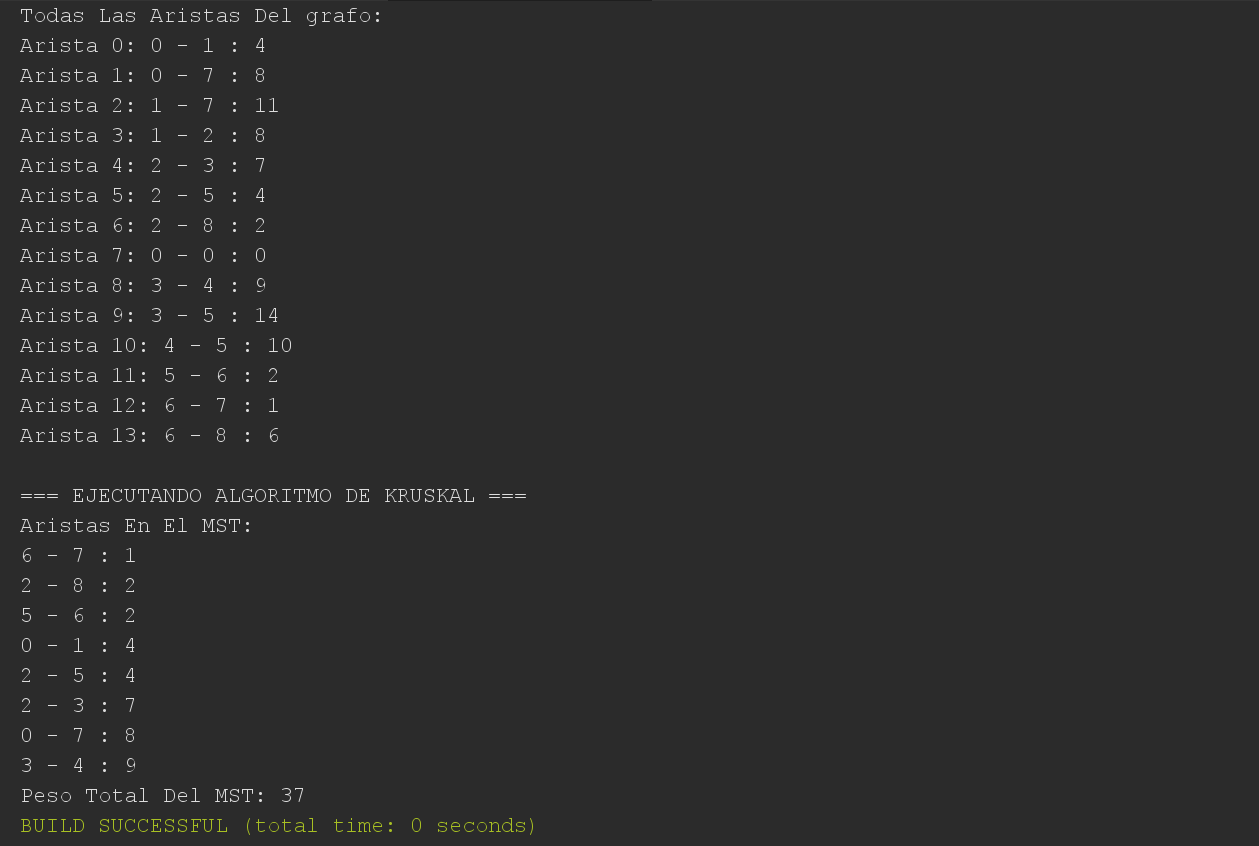
\includegraphics[width=1.0\textwidth]{image_2.png}
\end{center}

\newpage

\vspace*{-1.0cm}

\section{Algoritmo Prim's}
\vspace*{-0.5cm}
\begin{lstlisting}[language=Java, caption= \textbf{Implementación Prim's}]
    public void agregarArista(int indice, int u, int v, int peso) {
        grafo[u][v] = peso;
        grafo[v][u] = peso; // porque es un grafo no dirigido
    }

    // el int del inicio es el valor del vertice donde queremos iniciar nuestro recorrido
    public void prims(int iniciarRecorridoGrafo) {

        System.out.println("Selecciono Iniciar Desde El Vertice " + iniciarRecorridoGrafo);

        boolean[] visitado = new boolean[V]; // vector  de tipo booleano para comprobar si el vertice fue visitado o no
        int[] menorPesoAris = new int[V]; // vector tipo entero para almacenar las aristas de menor peso
        int[] padre = new int[V];

        Arrays.fill(menorPesoAris, Integer.MAX_VALUE);
        menorPesoAris[iniciarRecorridoGrafo] = 0;
        padre[iniciarRecorridoGrafo] = -1;

        for (int i = 0; i < V - 1; i++) {
            int u = minKey(menorPesoAris, visitado);
            visitado[u] = true;

            for (int v = 0; v < V; v++) {
                if (grafo[u][v] != 0 && !visitado[v] && grafo[u][v] < menorPesoAris[v]) {
                    padre[v] = u;
                    menorPesoAris[v] = grafo[u][v];
                }
            }
        }

        imprimirMST(padre);
    }

    private int minKey(int[] key, boolean[] visitado) {
        int min = Integer.MAX_VALUE, idx = -1;

        for (int i = 0; i < V; i++)
            if (!visitado[i] && key[i] < min) {
                min = key[i];
                idx = i;
            }

        return idx;
    }

   private void imprimirMST(int[] padre) {

    System.out.println("Aristas Usando Prims:");

    for (int i = 0; i < V; i++) {
        if (padre[i] != -1) {
            System.out.println(padre[i] + " - " + i + "  peso: " + grafo[i][padre[i]]);
        }
    }
}
   }

\end{lstlisting}

\vspace*{-0.5cm}
\begin{lstlisting}[language=Java, caption= \textbf{Main Implementación Prim's}]
        GrafoAlgoritmoPrims g = new GrafoAlgoritmoPrims(9);
        g.agregarArista(0, 0, 1, 4);   // A-B
        g.agregarArista(1, 0, 7, 8);   // A-H
        g.agregarArista(2, 1, 7, 11);  // B-H
        g.agregarArista(3, 1, 2, 8);   // B-C
        g.agregarArista(4, 2, 3, 7);   // C-D
        g.agregarArista(5, 2, 5, 4);   // C-F
        g.agregarArista(6, 2, 8, 2);   // C-I
        g.agregarArista(7, 3, 4, 9);   // D-E
        g.agregarArista(8, 3, 5, 14);  // D-F
        g.agregarArista(9, 4, 5, 10);  // E-F
        g.agregarArista(10, 5, 6, 2);  // F-G
        g.agregarArista(11, 6, 7, 1);  // G-H
        g.agregarArista(12, 6, 8, 6);  // G-I
        g.prims(6);  // iniciar en G (índice 6)
\end{lstlisting}

\noindent
El método agregarArista(int u, int v, int peso) se usa para construir el grafo en una matriz de adyacencia, asignando el mismo peso en grafo[u][v] y grafo[v][u] porque el grafo es no dirigido. Luego, el método prims(int iniciarRecorridoGrafo) implementa el algoritmo de Prim para hallar el árbol de expansión mínima (MST) empezando desde el vértice indicado: crea un arreglo visitado para saber qué vértices ya están en el MST, un arreglo menorPesoAris donde guarda el menor peso conocido para conectar cada vértice al árbol, y un arreglo padre que registra desde qué vértice se llega a cada nodo dentro del MST. Inicialmente pone todos los valores de menorPesoAris en infinito y al vértice de inicio le asigna 0 para que sea el primero en ser elegido. En cada iteración, la función auxiliar minKey selecciona el vértice no visitado con menor valor en menorPesoAris, lo marca como visitado y, recorriendo sus vecinos, actualiza menorPesoAris[v] y padre[v] si encuentra una arista de menor peso para llegar a ellos. Al final, el método imprimirMST(int[] padre) recorre el arreglo padre e imprime, para cada vértice con padre distinto de -1, la arista padre[i] - i junto con su peso, mostrando así las aristas que forman el árbol de expansión mínima obtenido con El Metodo Prim's.

\begin{center}
  \textbf{Ejecución Algortimo Usando Grafo Diapositivas CapL3 Pagina 98} \\
  \vspace*{0.5cm}
  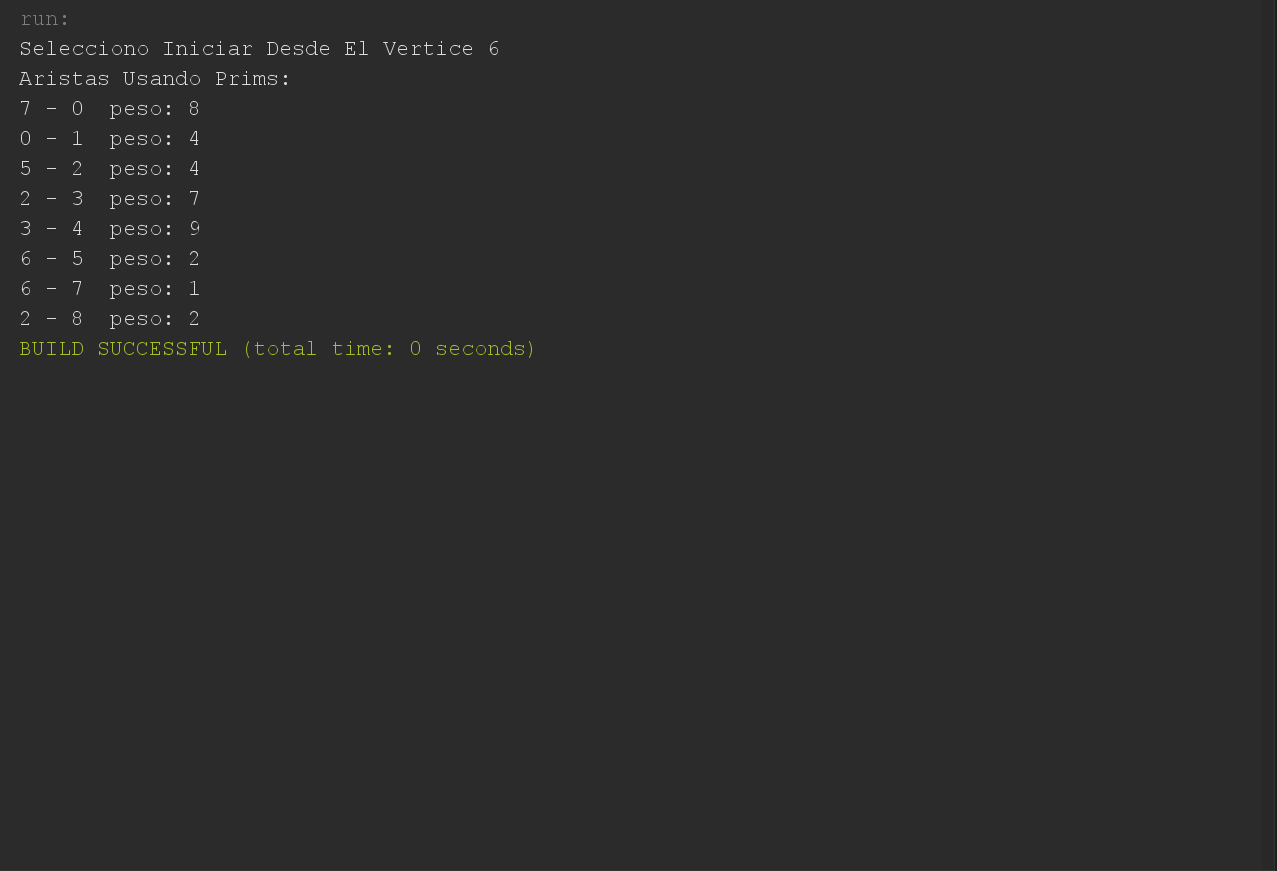
\includegraphics[width=1.0\textwidth]{image_3.png}
\end{center}

\section{Algoritmo Dijkstra}

\begin{lstlisting}[language=Java, caption= \textbf{Implementación Dijkstra}]
 // Constructor: crear un grafo con V vértices
    public GrafoAlgoritmoDijkstra(int V) {
        this.V = V;
        grafo = new int[V][V];

        // Inicializar matriz: 0
        for (int i = 0; i < V; i++) {
            for (int j = 0; j < V; j++) {
                if (i == j) {
                    grafo[i][j] = 0;
                } else {
                    grafo[i][j] = INF;
                }
            }
        }
  }

    // Agregar arista u–v con peso
    public void agregarArista(int u, int v, int peso) {
        grafo[u][v] = peso;
        grafo[v][u] = peso;
    }

    // Algoritmo de Dijkstra desde el vértice 'inicio' que seleccione
    public void dijkstra(int inicio) {
        int[] dist = new int[V];
        boolean[] visitado = new boolean[V];

        // Inicializar distancias
        for (int i = 0; i < V; i++) {
            dist[i] = INF;
            visitado[i] = false;
        }
        dist[inicio] = 0;

        // Repetir V-1 veces
        for (int c = 0; c < V - 1; c++) {

            // Escoger el vértice no visitado con menor distancia
            int u = nodoDistanciaMinima(dist, visitado);
            if (u == -1) break;
            visitado[u] = true;

            for (int v = 0; v < V; v++) {
                if (!visitado[v] &&
                    grafo[u][v] != INF &&
                    dist[u] != INF &&
                    dist[u] + grafo[u][v] < dist[v]) {

                    dist[v] = dist[u] + grafo[u][v];
                }
            }
        }

        imprimirDistancias(dist, inicio);
    }

    // Devuelve el índice del vértice no visitado con menor distancia
    public int nodoDistanciaMinima(int[] dist, boolean[] visitado) {
        int min = INF;
        int idx = -1;

        for (int i = 0; i < V; i++) {
            if (!visitado[i] && dist[i] < min) {
                min = dist[i];
                idx = i;
            }
        }
        return idx;
    }

    // Imprimir las distancias desde el vértice inicio
    public void imprimirDistancias(int[] dist, int inicio) {
        System.out.println("Distancias Mas Cortas Desde El Vertice " + inicio + ":");
        for (int i = 0; i < V; i++) {
            if (dist[i] == INF) {
                System.out.println(inicio + " -> " + i + " = INF");
            } else {
                System.out.println(inicio + " -> " + i + " = " + dist[i]);
            }
        }
    }
}
\end{lstlisting}

\begin{lstlisting}[language=Java, caption= \textbf{Main Implementación Dijkstra}]
     // El grafo tiene 9 vértices (A=0, B=1, ..., I=8)
        GrafoAlgoritmoDijkstra g = new GrafoAlgoritmoDijkstra(9);

        g.agregarArista(0, 1, 4);   // A-B
        g.agregarArista(0, 7, 8);   // A-H
        g.agregarArista(1, 7, 11);  // B-H
        g.agregarArista(1, 2, 8);   // B-C
        g.agregarArista(2, 3, 7);   // C-D
        g.agregarArista(2, 5, 4);   // C-F
        g.agregarArista(2, 8, 2);   // C-I
        g.agregarArista(3, 4, 9);   // D-E
        g.agregarArista(3, 5, 14);  // D-F
        g.agregarArista(4, 5, 10);  // E-F
        g.agregarArista(5, 6, 2);   // F-G
        g.agregarArista(6, 7, 1);   // G-H
        g.agregarArista(6, 8, 6);   // G-I

        // Ejecutando Dijkstra desde el vértice 0 (A)
        g.dijkstra(0);
    }
}

\end{lstlisting}

\begin{center}
  \textbf{Ejecución Algortimo Usando Grafo Diapositivas CapL3 Pagina 100}
  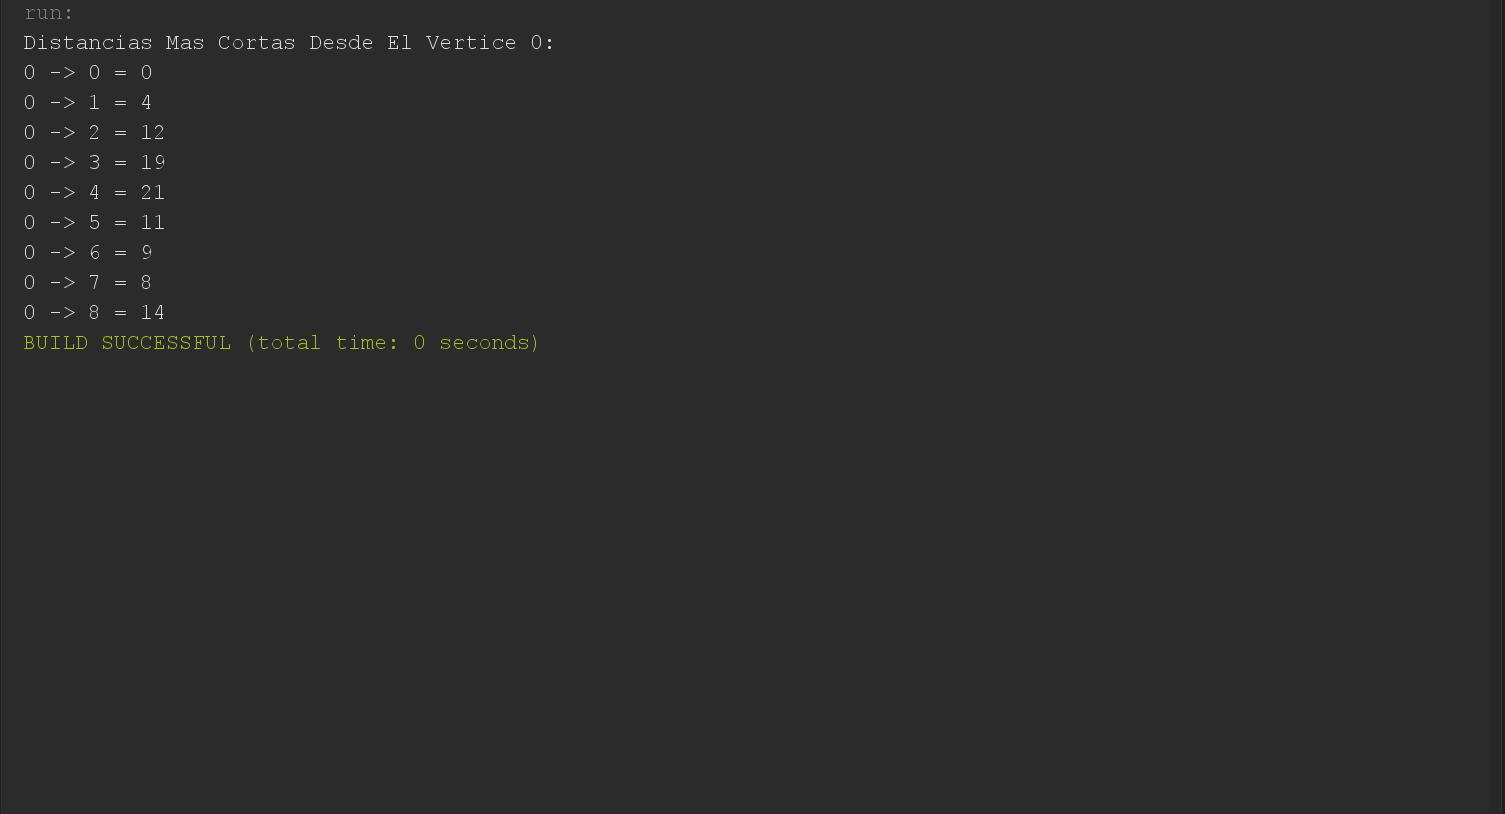
\includegraphics[width=1.0\textwidth]{image_4.png}
\end{center}

El algorimito Dijkstra, usa la matriz de adyacencia para la correcta representación del grafo respectivamente. Primero se define un valor “INF” que funciona como infinito, indicando que entre dos vértices no existe conexión directa. Al crear el grafo, la matriz se inicializa colocando 0 cuando un vértice es igual a sí mismo y colocando INF cuando no existe arista entre ellos. Despues con ayuda del metodo agregarArista() permite añadir una arista entre dos vértices u y v asignando el peso en la direccion adecuada. se crea una matriz que nos servira para las distancias y los visitados, todas las distancias se inicializan en infinito excepto la del vértice inicial, que queda en 0. Luego se repite el proceso de seleccionar el vértice no visitado con la distancia más pequeña, gracias al método nodoDistanciaMinima. Ese vértice se marca como visitado y se revisan todos sus vecinos para actualizar (relajar) la distancia si pasar por ese vértice mejora el camino. Estas actualizaciones se realizan hasta recorrer todos los vértices. Finalmente, el método imprimirDistancias muestra la distancia mínima desde el vértice inicial hacia cada vértice del grafo, mostrando “INF” cuando algún vértice no puede alcanzarse. En conjunto, el código construye un grafo, permite agregar aristas y calcula las rutas más cortas desde un nodo origen usando el algoritmo de Dijkstra de forma eficiente y ordenada.

\newpage

\section{Algoritmo Floyd-Warshall}

\begin{lstlisting}[language=Java, caption= \textbf{Implementación FloydWarshall}]
    public GrafoAlgoritmoFloydWarshall(int V) {
        this.V = V;
        dist = new int[V][V];

        for (int i = 0; i < V; i++) {
            for (int j = 0; j < V; j++) {
                if (i == j) dist[i][j] = 0;
                else dist[i][j] = INF;
            }
        }
    }

    // Agregar arista u–v con pesos
    public void agregarArista(int u, int v, int peso) {
        dist[u][v] = peso;
        dist[v][u] = peso; 
    }

    // Algoritmo Floyd–Warshall
    public void floydWarshall() {
        for (int k = 0; k < V; k++) {        // vértice intermedio
            for (int i = 0; i < V; i++) {    // fila
                for (int j = 0; j < V; j++) { // columna
                    if (dist[i][k] + dist[k][j] < dist[i][j]) {
                        dist[i][j] = dist[i][k] + dist[k][j];
                    }
                }
            }
        }
    }

    // Imprimir matriz
    public void imprimirDistancias() {
        System.out.println("Matriz de distancias más cortas:");
        for (int i = 0; i < V; i++) {
            for (int j = 0; j < V; j++) {
                if (dist[i][j] == INF) System.out.print("INF ");
                else System.out.print(dist[i][j] + " ");
            }
            System.out.println();
        }
    }
}
\end{lstlisting}

\newpage

\begin{lstlisting}[language=Java, caption= \textbf{Main Implementación FloydWarshall}]
        public static void main(String[] args) {

        // El grafo que se usa tiene 9 vértices: 0 a 8
        GrafoAlgoritmoFloydWarshall g = new GrafoAlgoritmoFloydWarshall(9);

        g.agregarArista(0, 1, 4);   // A-B
        g.agregarArista(0, 7, 8);   // A-H
        g.agregarArista(1, 7, 11);  // B-H
        g.agregarArista(1, 2, 8);   // B-C
        g.agregarArista(2, 3, 7);   // C-D
        g.agregarArista(2, 5, 4);   // C-F
        g.agregarArista(2, 8, 2);   // C-I
        g.agregarArista(3, 4, 9);   // D-E
        g.agregarArista(3, 5, 14);  // D-F
        g.agregarArista(4, 5, 10);  // E-F
        g.agregarArista(5, 6, 2);   // F-G
        g.agregarArista(6, 7, 1);   // G-H
        g.agregarArista(6, 8, 6);   // G-I

        // Ejecutar Floyd–Warshall
        g.floydWarshall();

        // Imprimir matriz final
        g.imprimirDistancias();
    }
}
\end{lstlisting}

\begin{center}
\textbf{Ejecución Algortimo Usando Grafo Diapositivas CapL3 Pagina 100}    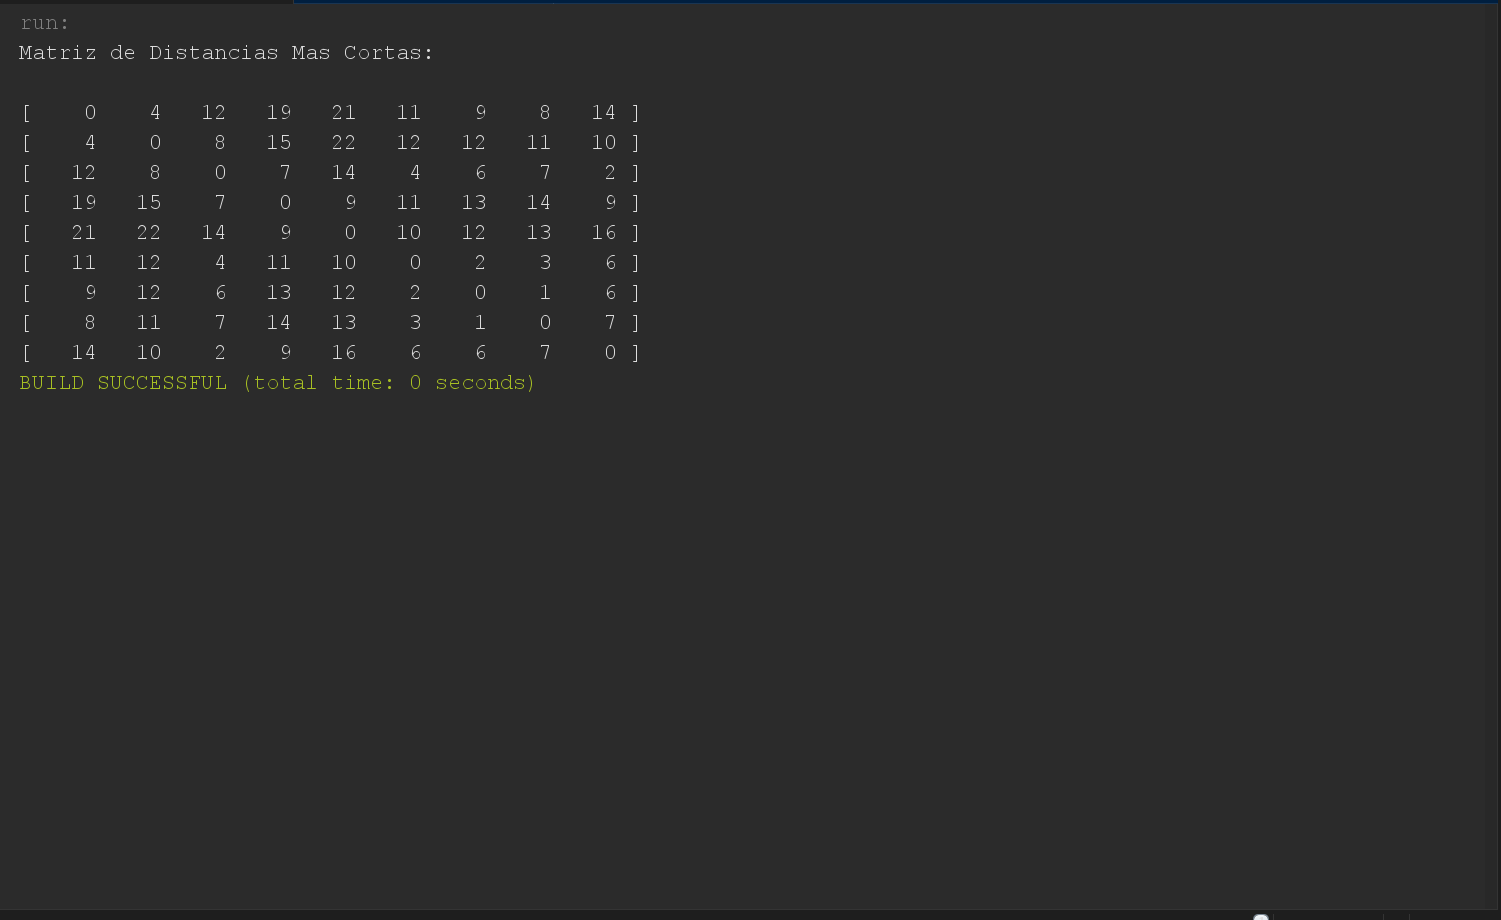
\includegraphics[width=0.8\textwidth]{image_5.png}
\end{center}

\newpage

  \vspace*{-1.0cm}
  \noindent
El algoritmo de Floyd–Warshall trabaja con una matriz de adyacencia, donde se coloca 0 cuando un vértice es igual a sí mismo y INF cuando no existe conexión directa. Con el método agregarArista() se actualizan en la matriz las distancias entre los vértices conectados.

Una vez inicializada la matriz, el algoritmo busca calcular las distancias más cortas entre todos los pares de vértices. Para ello, prueba cada vértice k como posible camino intermedio entre los vértices i y j. Si pasar por k entonces se ofrece una ruta más corta que la registrada actualmente, la matriz se actualiza con ese nuevo valor, tantas veces sea posible, logrando que la matriz final contenga las rutas mínimas entre cualquier par de nodos del grafo.

Finalmente, imprimirDistancias() muestra la matriz resultante, utilizando “INF” cuando dos vértices siguen sin tener una ruta posible.

\end{document}